A 3d-printed case was designed in Solidworks and constructed using a common 3d-printer. The results are shown in \autoref{fig:caseV1_fitted}. \par
\begin{figure}[h]
    \centering
    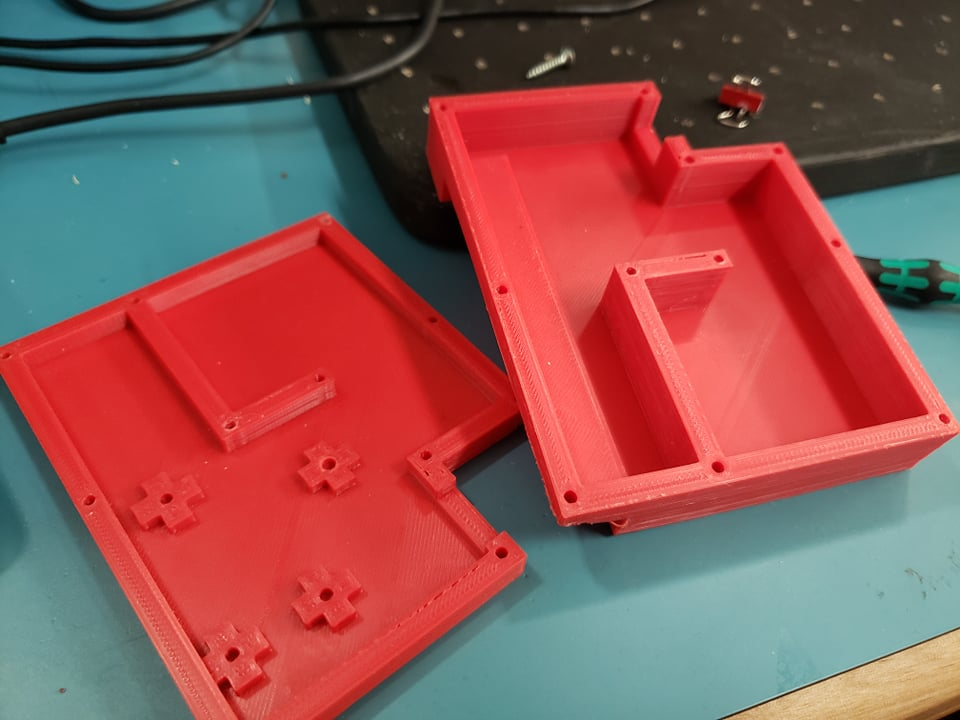
\includegraphics[width=0.4\textwidth]{caseV1_topandbottom}
    \caption{3d-printed case top and bottom.}
    \label{fig:caseV1_topandbottom}
\end{figure}
\begin{figure}[h]
    \centering
    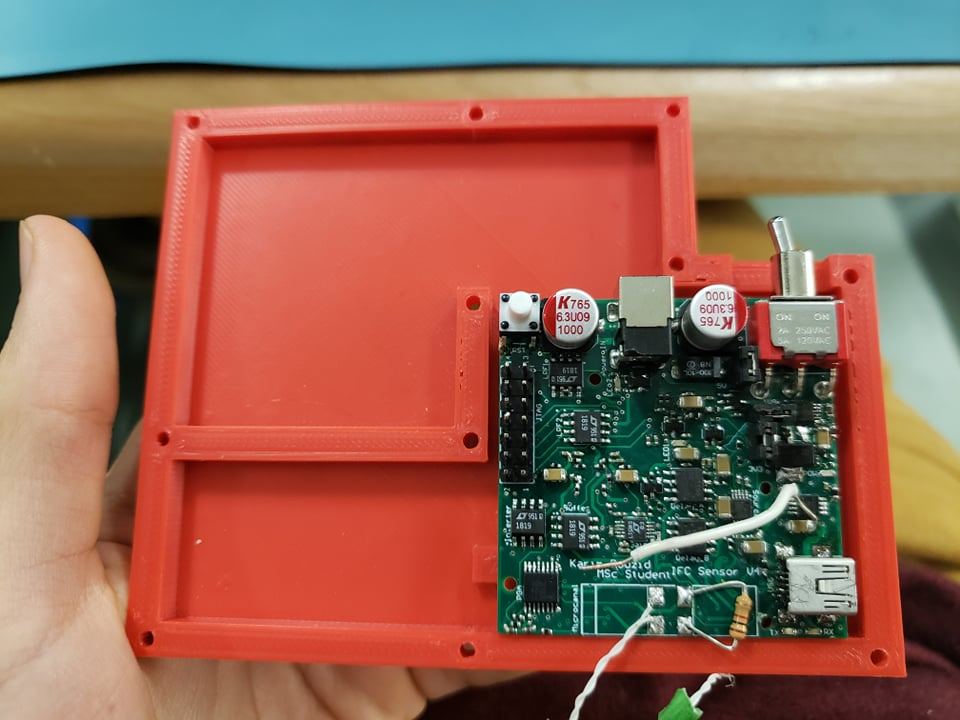
\includegraphics[width=0.4\textwidth]{caseV1_fitted}
    \caption{3d-printed case fitted with the PCB.}
    \label{fig:caseV1_fitted}
\end{figure}
